% CVPR 2023 Paper Template
% based on the CVPR template provided by Ming-Ming Cheng (https://github.com/MCG-NKU/CVPR_Template)
% modified and extended by Stefan Roth (stefan.roth@NOSPAMtu-darmstadt.de)
\documentclass[10pt,twocolumn,letterpaper]{article}

%%%%%%%%% PAPER TYPE  - PLEASE UPDATE FOR FINAL VERSION
% \usepackage[review]{cvpr}      % To produce the REVIEW version
\usepackage{cvpr}              % To produce the CAMERA-READY version
%\usepackage[pagenumbers]{cvpr} % To force page numbers, e.g. for an arXiv version


\usepackage{CJKutf8} % For chinese output

% Include other packages here, before hyperref.
\usepackage{graphicx}
\usepackage{amsmath}
\usepackage{amssymb}
\usepackage{booktabs}
\usepackage{xcolor}
\graphicspath{ {./images/} }

% It is strongly recommended to use hyperref, especially for the review version.
% hyperref with option pagebackref eases the reviewers' job.
% Please disable hyperref *only* if you encounter grave issues, e.g. with the
% file validation for the camera-ready version.
%
% If you comment hyperref and then uncomment it, you should delete
% ReviewTempalte.aux before re-running LaTeX.
% (Or just hit 'q' on the first LaTeX run, let it finish, and you
%  should be clear).
\usepackage[pagebackref,breaklinks,colorlinks]{hyperref}


% Support for easy cross-referencing
\usepackage[capitalize]{cleveref}
\crefname{section}{Sec.}{Secs.}
\Crefname{section}{Section}{Sections}
\Crefname{table}{Table}{Tables}
\crefname{table}{Tab.}{Tabs.}


%%%%%%%%% PAPER ID  - PLEASE UPDATE
\def\cvprPaperID{*****} % *** Enter the CVPR Paper ID here
\def\confName{CVPR}
\def\confYear{2023}


\begin{document}
\begin{CJK*}{UTF8}{bsmi}

%%%%%%%%% TITLE - PLEASE UPDATE
\title{Google - Isolated Sign Language Recognition}

\author{王浩 \\
國立成功大學 資訊工程學系\\
F74082141\\
{\tt\small Howard.H.Wang.23@gmail.com}
% For a paper whose authors are all at the same institution,
% omit the following lines up until the closing ``}''.
% Additional authors and addresses can be added with ``\and'',
% just like the second author.
% To save space, use either the email address or home page, not both
\and
杜孟聰\\
國立成功大學 資訊工程學系\\
F74082028\\
{\tt\small F74082028@gs.ncku.edu.tw}
}
\maketitle

%%%%%%%%% ABSTRACT
\begin{abstract}
   This paper aims to classify isolated American Sign Language (ASL) signs using a deep learning model. 
   To achieve this, we trained the model on labeled landmark data extracted via the MediaPipe Holistic Solution. 
   Our approach leverages the accuracy and reliability of this technology to enhance the robustness of the model and improve its performance. 
   By accurately classifying ASL signs, our method has the potential to support individuals with hearing impairments and 
   enable better communication between hearing and non-hearing populations.
\end{abstract}

%%%%%%%%% BODY TEXT
\section{Introduction}
\label{sec:intro}
Deaf children born to hearing parents are at risk of Language Deprivation Syndrome if they don't have access to a fully developed language early in life. 
However, learning American Sign Language (ASL) can be time-consuming and resource-intensive for parents. 
Automatic sign language recognition technology can help overcome this barrier by recognizing and translating signs into text or speech.

In this paper, we propose a novel approach to isolated sign language recognition using computer vision techniques and machine learning algorithms. 
Our approach improves accuracy, robustness, and speed, as demonstrated on a publicly available dataset.

{\color{blue} this 
is the test for change 
color}

%-------------------------------------------------------------------------
\subsection{American Sign Language}

American Sign Language (ASL) is a language used primarily by members of the Deaf community in North America. 
It is not a visual representation of English, but has its own unique grammar, syntax, and vocabulary. 
ASL is a visual-gestural language, meaning that it uses facial expressions, body language, and hand movements to convey meaning.

\subsection{Isolated Sign Language Recognition}

ISLR stands for Isolated Sign Language Recognition, which is the task of recognizing individual signs or tokens called glosses from a given segment of signing video clip.
It is the process of recognizing sign language gestures performed by a person in isolation, without considering the context or the surrounding gestures. 
We will train a machine learning model that can accurately recognize isolated sign language signs and classify them into the correct sign category.

%------------------------------------------------------------------------
\section{System framwork}
\label{sec:formatting}

We will use the raw data extracted from the MediaPipe Holistic Solution, which records every movement in video by landmark.
Based on that data, we use an ensamble model to train a deep learning model for classifying isolated American Sign Language (ASL) signs.

%-------------------------------------------------------------------------
\subsection{Data Type}
MediaPipe Holistic Solution~\cite{https://doi.org/10.48550/arxiv.1906.08172} is a powerful, easy-to-use software tool that can detect and track multiple human body parts and gestures in real-time video streams. 
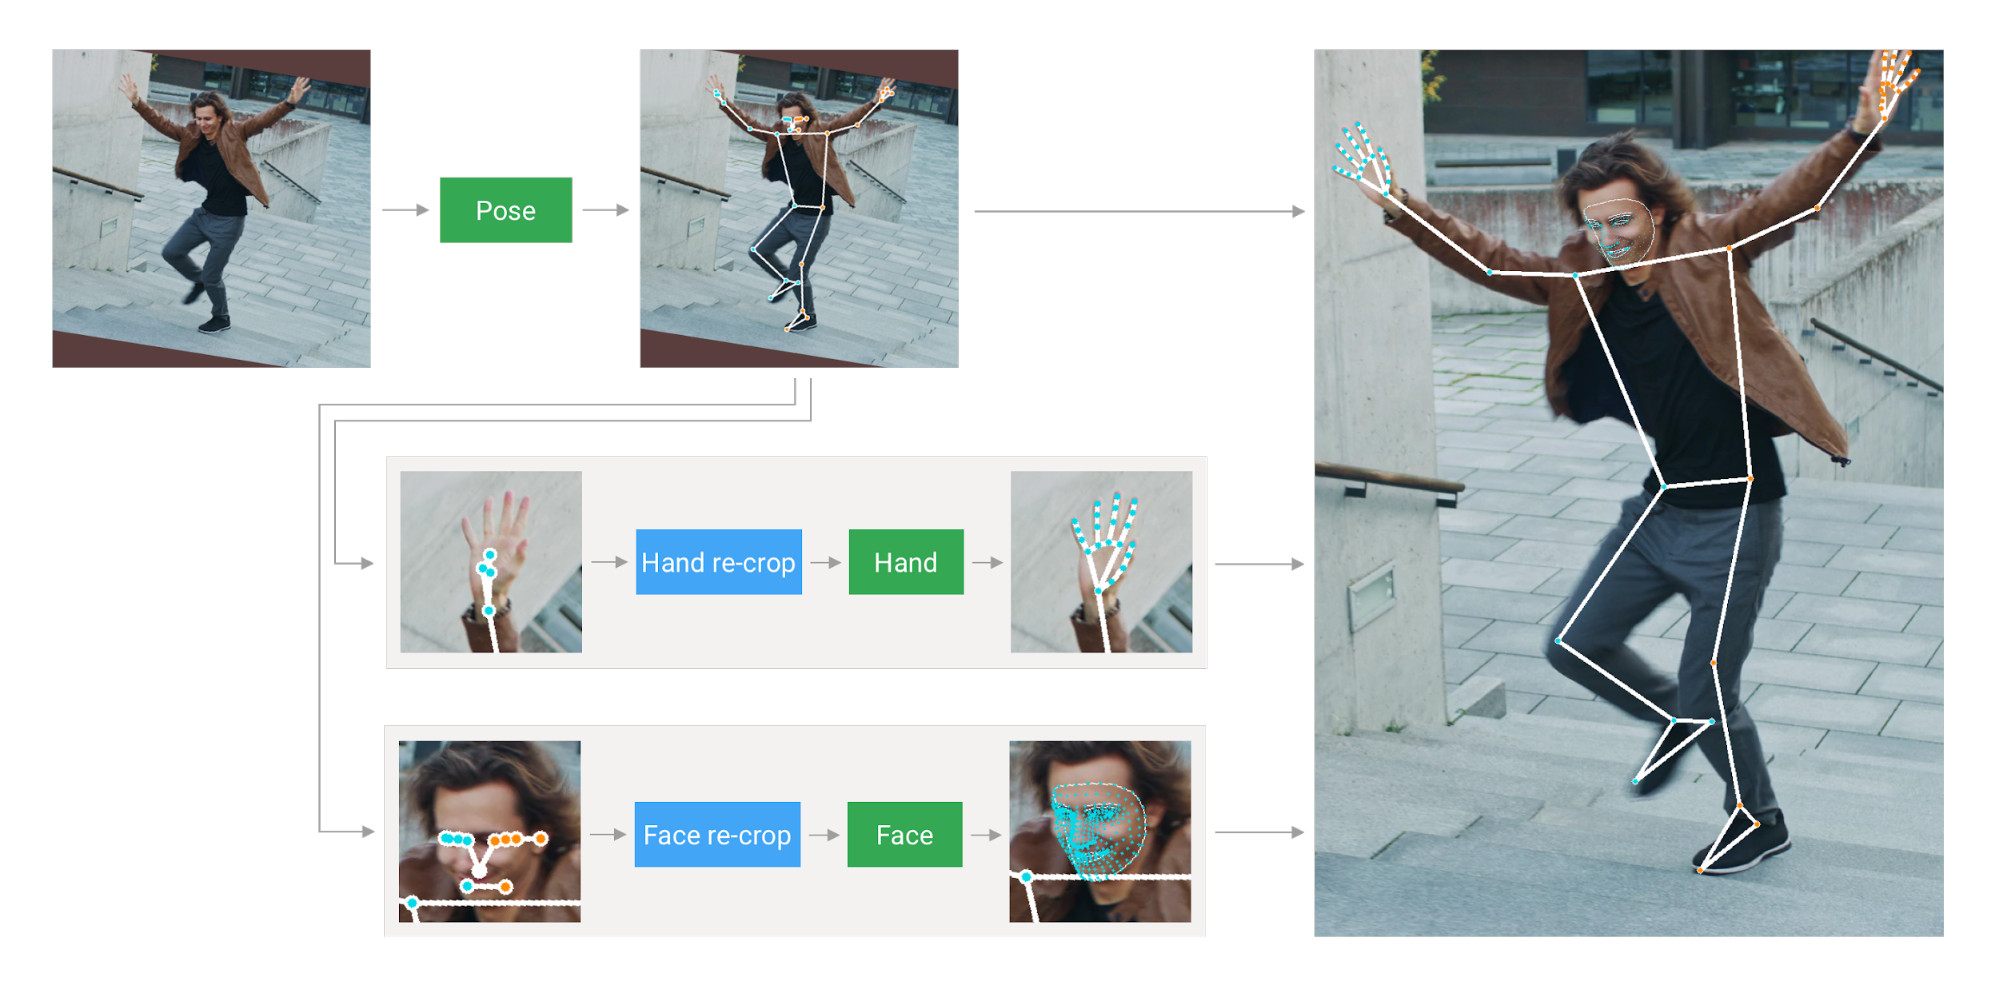
\includegraphics[width=80mm]{holistic_pipeline_example}
The way that MediaPipe Holistic Solution records facial expressions, body language, and hand movements is by using landmarks.

Landmarks or keypoints are like dots that are placed on important areas of an object or a person's body. 
These dots help a computer to understand where these important areas are and how they are moving.

%------------------------------------------------------------------------
\subsection{Model}

Our proposed model leverages a simple linear architecture with added activation functions to form 
the foundation of our approach. To enhance the model's performance, we will modify the input data format, 
taking into consideration the unique properties of facial expressions, body language, and hand movements.
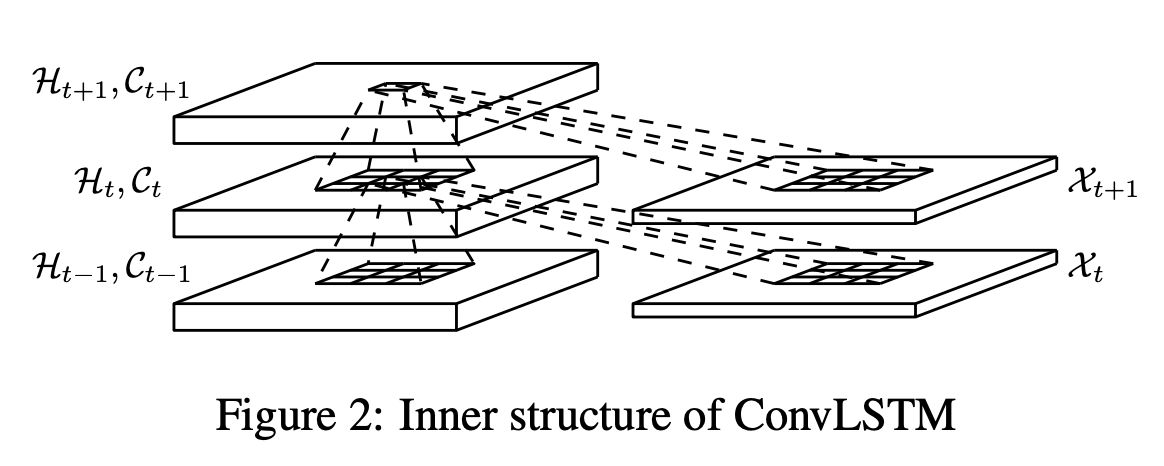
\includegraphics[width=80mm]{ConvLSTM}
In addition, we will explore the use of time-series models and convolution-based models, 
such as ConvLSTM~\cite{NIPS2015_07563a3f}, to identify the optimal model for fitting the features present in our video-captured frame data. 
By evaluating multiple model architectures and comparing their effectiveness, 
we aim to select the most robust and efficient approach for our isolated American Sign Language (ASL) sign recognition task.

Our model development process is designed to enhance the accuracy and reliability of our approach, 
thereby improving the overall quality of our results. 
Through a comprehensive evaluation of various model architectures, we aim to establish a state-of-the-art ASL sign recognition system 
that can effectively support communication between deaf and hearing populations.

%------------------------------------------------------------------------
\section{Expected Result}
Our proposed state-of-the-art model, which utilizes the input data of every video frame's landmarks captured by the MediaPipe Holistic Solution, 
is expected to significantly improve the accuracy and speed of isolated sign language recognition. 
We anticipate that the model will achieve high recognition rates for individual signs, 
thus aiding in the communication and language acquisition process of individuals who are deaf or hard of hearing. 
We believe that our research will contribute to the development of more sophisticated and efficient sign language recognition technology, 
making communication more accessible for the Deaf community


%%%%%%%% REFERENCES
{\small
\bibliographystyle{ieee_fullname}
\bibliography{egbib}
}

\end{CJK*}
\end{document}

